\section{Optimization Algorithm} \label{sct: opt_alg}
Recall that we are optimizing the problem with the following form:
\begin{align}\label{constraint opt}
   \beta_n(M) = \arg\max_{\beta:\ \|\beta\|_1 \leq M} \sum_{i=1}^{n} \sum_{j=1}^{n+k+1} \beta_j \phi_j(x_i) - n\log C(\beta), 
\end{align} 
and its Lagrangian form is as follows:
\begin{align} \label{lag opt}
   \beta_n(M) = \arg\max_{\beta} \sum_{i=1}^{n} \sum_{j=1}^{n+k+1} \beta_j \phi_j(x_i) - n\log C(\beta) - \lambda \|\beta\|_1, 
\end{align} 

Tuning the upper bound $M$ of the $L_1$ norm in the constraint form is more statistically meaningful, because the final choice of $M$ should reflect the magnitude of the SVN of the truth. However, we prefer the Lagrangian form because the algorithm for the constraint form always involves projection to the $L_1$ ball. In practice, we find that soft thresholding provides a more robust dimension reduction through iterations than projection to the $L_1$ ball.

\subsection{Candidate Algorithms} \label{subsct: cand_alg}
While generic convex solvers such as \texttt{MOSEK}, \texttt{ECOS}, or \texttt{SCS} within the \texttt{CVXPY} package can, in principle, handle our convex optimization problem, their general strategy is to map any instance into a conic programming framework. This approach, though flexible, is not tailored to the structural features of our estimator. Moreover, as the sample size increases to the range of 3,000–5,000 observations, we find that the default knot point selection of these solvers becomes less effective: a large number of unnecessary knot points remain active, primarily due to accuracy constraints in the optimization process. A demonstration of this is shown in Figure~\ref{fig:opt-algorithms-tn}. These limitations motivate the development of specialized algorithms that exploit the structure of the problem and incorporate effective knot point selection strategies, yielding both improved scalability and enhanced statistical efficiency. 

We refer to the matrix of initiated basis evaluated at the data points as the basis matrix. The basis matrix is an $n \times (n+k+1)$ matrix. 
\paragraph{Standard Algorithm:} When using the truncated power basis, the Hessian constructed from the basis matrix is usually ill-conditioned and thus first-order methods like Fast Iterative Shrinkage-Thresholding Algorithm (FISTA) would converge slowly in iterations. Therefore, we propose a standard algorithm combining proximal Newton's method and the coordinate descent algorithm. An advantage of proximal Newton is that we can calculate the Hessian in closed form. Also, we could warm start the algorithm when using cross-validation to choose $\lambda$ in order to keep Newton's method within the quadratic convergence range. 

\paragraph{Large-scale Adjustment:} The proximal Newton's method fails for large-scale problems due to memory issues. When the sample size n is too large, such as 10,000 or 100,000, the initialized Hessian will be $O(n^2)$ and too large to be memorized. For this problem, we propose the Quasi-Newton method (L-BFGS) and coordinate descent. An easy implementation is just memorizing the most recent pair of differences in parameters and their corresponding gradient. Thus, the approximation of the Hessian is a scaled identity matrix, and we update the scale at each iteration. The memory reduces from $O(n^2)$ to $O(n)$. Pragmatically, we find out that including the coordinate descent is more robust for large-scale problems.

Another algorithm we propose is a variant of AdaGrad using the inner product defined in Equation~\ref{eq:inner-product-score}. We just compute the diagonal entries of the Hessian for each iteration. Thus, the cost per iteration becomes very cheap, and the memory is just $O(n)$ and totally affordable. 

\begin{remark}
The development of the large-scale methods seems to be unnecessary in the univariate case, because, in HAL theory like Appendix~\ref{appB: $L^2$ Convergence Analysis} and Appendix~\ref{appendix_E: Uniform Convergence Rate}, we only need about $O^+(n^{\frac{1}{2k+3}})$ knots, and we could choose them based on the percentile of the original sample while remaining the performance. However, in the multivariate case, we need such algorithms because (1) the definition of multivariate percentile could be meaningless and (2) even a small sample size could initialize a large number of parameters $n(2^d - 1)$ for $ d$-dimensional data.
\end{remark}

\subsection{Exploration of Optimization Algorithms} \label{subsct: exploration_of_optimization_algorithms}
We study the performance of the optimization algorithms in some fixed settings where \texttt{CVXPY} solvers have trouble selecting knot points. We here demonstrate the performance of the optimization algorithms on the Truncated Normal Data Generating Process (DGP), and the visualizations are shown in Figure~\ref{fig:opt-algorithms-tn}. We use the final result of \texttt{CVXPY} solutions as the baseline, and we evaluate the performance of the optimization algorithms by comparing the knot selection and loss convergence per iteration and per FLOP. The FLOPs are estimated by the computational complexity of the algorithms, which is shown in Table~\ref{tab:complexity-summary}. Additional results for all six DGPs and the reasoning of the computational complexity based on our implementation is provided in Appendix~\ref{app:knot-selection}.

\begin{table}[H]
   \centering
   \begin{tabular}{ll}
   \toprule
   Algorithm & Dominant per-iteration complexity \\
   \midrule
   FISTA & $\Theta\big((n + G)\,K\big)$ \\
   Proximal AdaGrad & $\Theta\big((n + G)\,K\big)$ \\
   Proximal Newton L\,-\,BFGS & $\Theta\big((1+L_k)\,(n + G)\,K\big)$ \\
   Proximal Newton (full) & $\Theta\big(G\,K^2 + s\,K^2\big) + \Theta\big((1+L_k)\,(n + G)\,K\big)$ \\
   \bottomrule
   \end{tabular}
   \caption{Dominant per\,-\,iteration computational complexity. Here $n$ is the number of samples, $G$ the number of midpoint intervals used for normalization, $K$ the number of basis coefficients, $s$ the active set size in coordinate descent, and $L_k$ the number of line\,-\,search objective evaluations at iteration $k$.}
   \label{tab:complexity-summary}
   \end{table}


\begin{figure}[H]
\centering
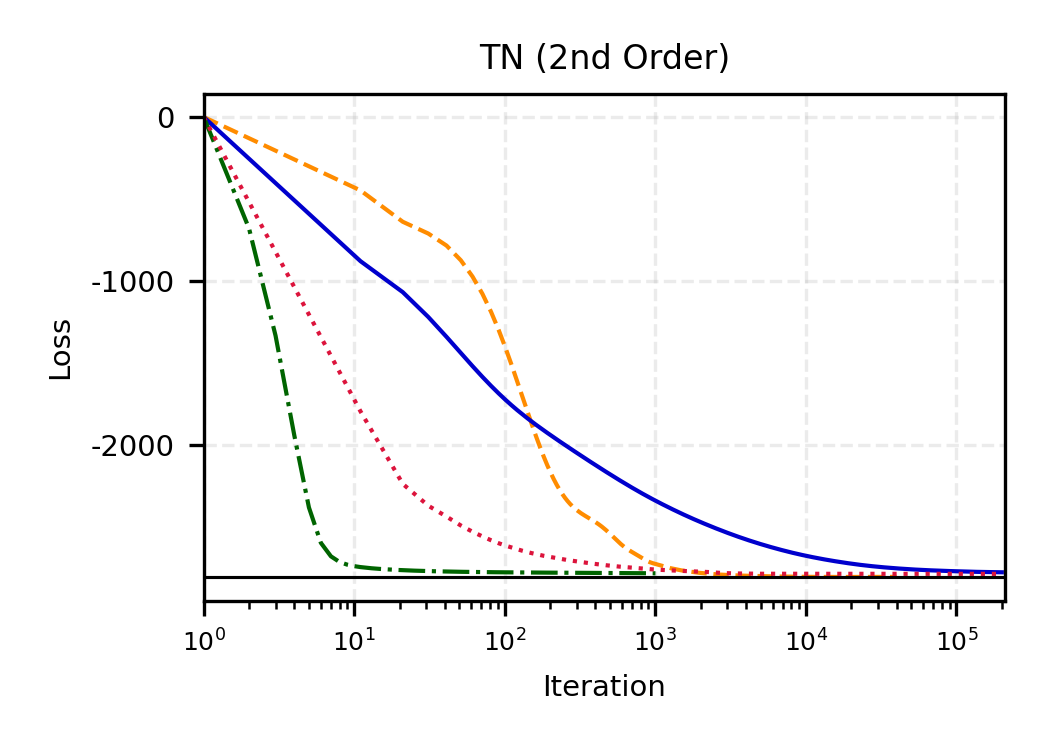
\includegraphics[width=.36\textwidth]{resources/optimization_algorithms/per_iter/TruncatedNormal_order_2_loss_per_iter.png}
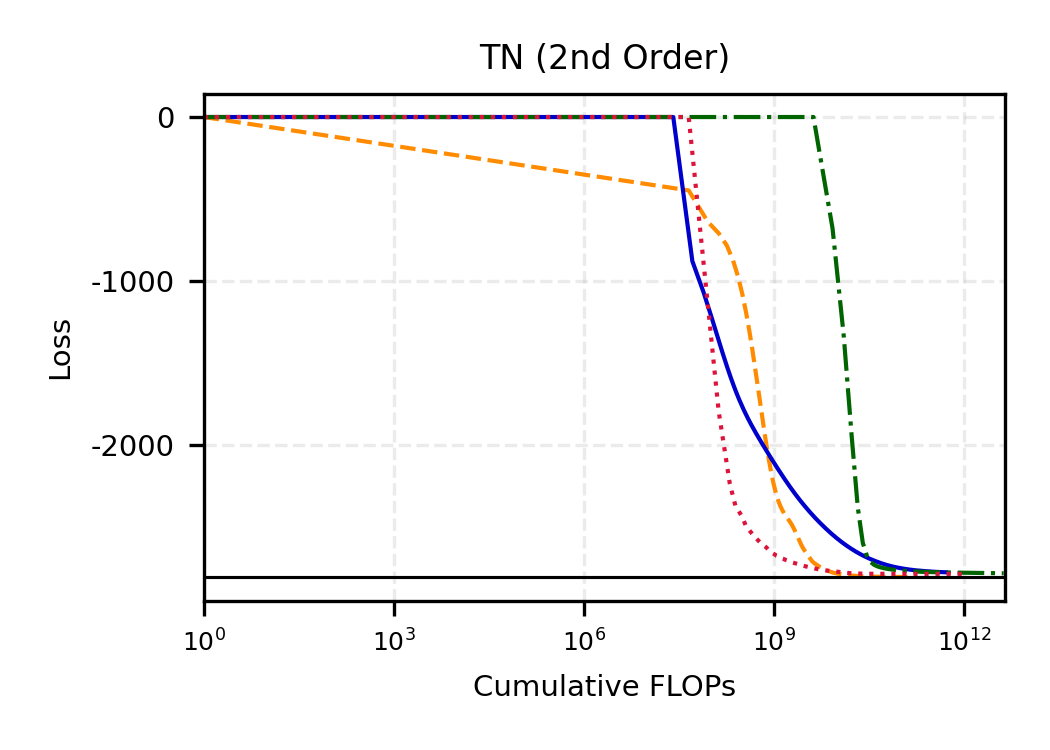
\includegraphics[width=.36\textwidth]{resources/optimization_algorithms/per_flop/TruncatedNormal_order_2_loss_per_flop.png}\\
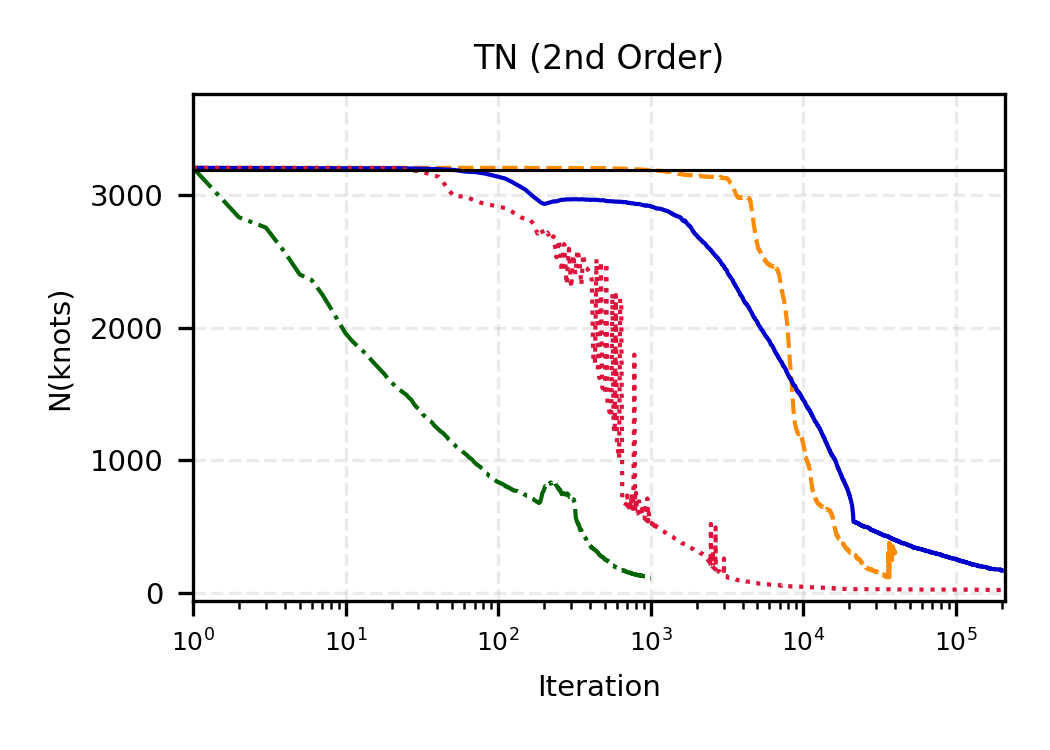
\includegraphics[width=.36\textwidth]{resources/optimization_algorithms/per_iter/TruncatedNormal_order_2_knot_selection.png}
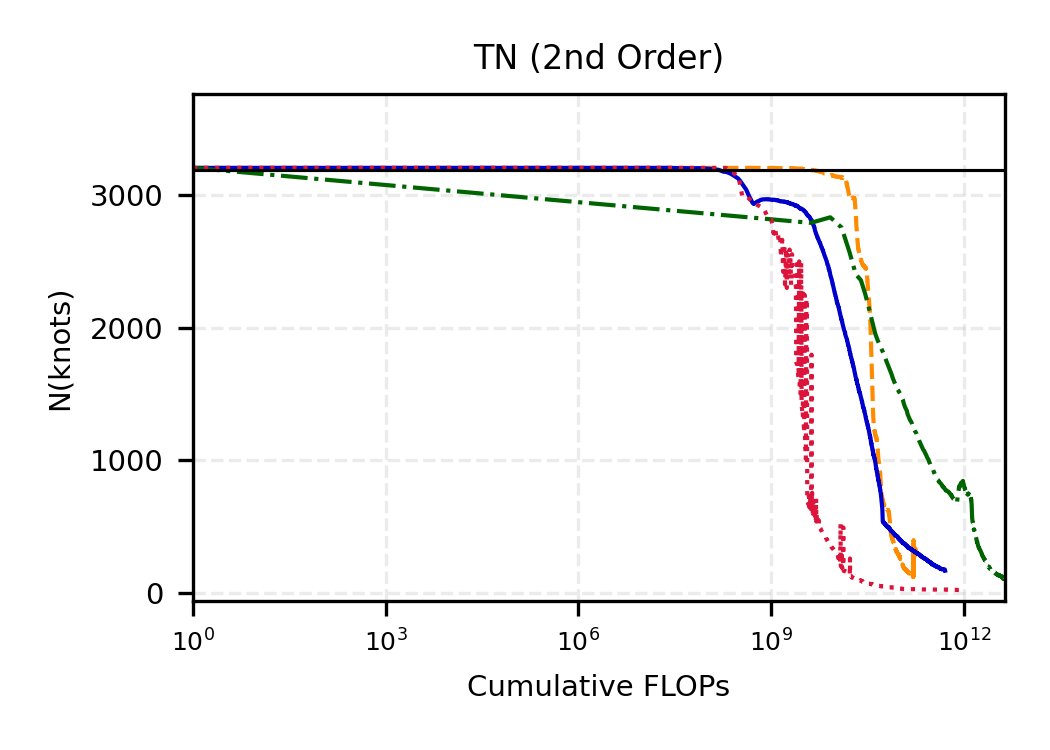
\includegraphics[width=.36\textwidth]{resources/optimization_algorithms/per_flop/TruncatedNormal_order_2_knot_selection_flops.png}\\
\vspace{-0.5em}

\includegraphics[width=.72\textwidth]{resources/optimization_algorithms/per_iter/legend_knot_selection_algorithms.png}
\caption{Optimization algorithm comparison for Truncated Normal (2nd order basis): knot selection per iteration (top left), knot selection per FLOP (top right), loss convergence per iteration (bottom left), and loss convergence per FLOP (bottom right).}
\label{fig:opt-algorithms-tn}
\end{figure}

Based on the results, we find that the Proximal Newton algorithm takes the fewest iterations to converge, and it is also efficient in selecting knot points, which is expected because it is a second-order method and we have the closed-form Hessian. The Proximal Newton L-BFGS algorithm is also efficient in selecting knot points, and it is more efficient than the Proximal Newton algorithm in terms of FLOPs. However, the Proximal Newton L-BFGS algorithm is sometimes unstable in the process of knot selection. AdaGrad is very fast and efficient, but in practice, we find that it has oscillatory behavior as well. FISTA is easy to implement and robust, but it is slow as expected in terms of iterations and wall-clock time. 

Generally speaking, comparing to the \texttt{CVXPY} solvers, the optimization algorithms we proposed succeed in selecting knot points and converging to the global optimum. This aligns with the HAL-MLE theory that we only need $O^+(n^{\frac{1}{2k+3}})$ knots to achieve the desired performance, and this also informs us that the numerical problem of \texttt{CVXPY} solvers is severe when the sample size is large. However, we cannot make a fair comparison between the optimization algorithms and the \texttt{CVXPY} solvers in terms of wall-clock time because some of the \texttt{CVXPY} solvers are closed-source and some are coded in C, whereas we coded our own solvers in Python.

\begin{remark}[Computational comparison with B-splines]
\label{rem:comp_comparison}
It is well known that locally supported B-splines can be more computationally efficient, with their primary advantage stemming from the banded structure of the Hessian matrix. However, this benefit diminishes a lot in large-scale problems where the full Hessian cannot be computed explicitly and must instead be approximated. In addition, for the large-scale problem, the jumping matrix associated with the variation penalty is difficult to track when knot points are chosen in a data-adaptive manner, especially with smoothness order $k \geq 1$. By contrast, the truncated power basis—though less efficient computationally—offers the simplest and most transparent representation of sectional variation, making it particularly well suited for our theoretical analysis and algorithmic development.
\end{remark}